\documentclass[convert]{standalone}
\usepackage[protrusion=false,expansion=false]{microtype}
\usepackage{mathpazo}

\usepackage[utf8]{inputenc}
\usepackage[T1]{fontenc}

\usepackage{tikz}
\usetikzlibrary{automata,arrows}

\begin{document}
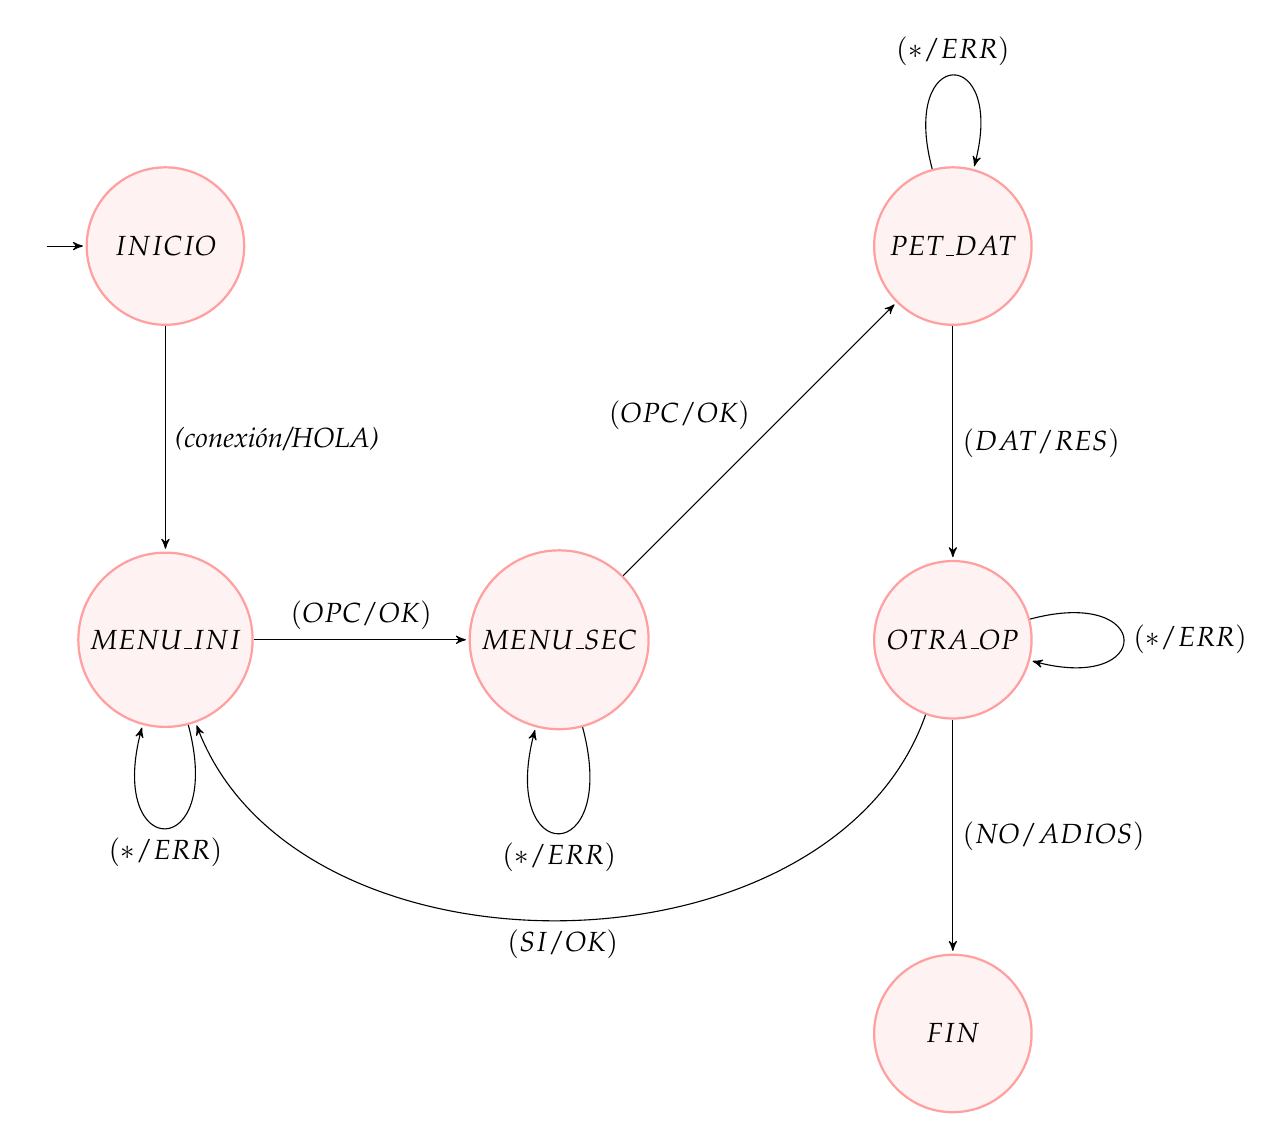
\begin{tikzpicture}[>=stealth',shorten >=1pt,auto,node distance=5 cm, scale = 1, transform shape, initial text=]
 \tikzstyle{state}=[circle,thick,draw=pink!150,fill=pink!20,minimum size=20mm]

\node[initial,state] (A)                               	 {$INICIO$};
\node[state]         (B) [below of=A]                    {$MENU\_INI$};
\node[state]         (C) [right of=B]             		 {$MENU\_SEC$};
\node[state]         (D) [right of=C]            		 {$OTRA\_OP$};
\node[state]         (E) [above of=D]             		 {$PET\_DAT$};
\node[state]         (F) [below of=D]            		 {$FIN$};

\path[->] 	(A) edge       	        node [align=center]  {\textit{(conexión/HOLA)}}(B)
			(B) edge [loop below]   node [align=center]  {$(*/ERR)$}        (B)
			(B) edge 		       	node [align=center]  {$(OPC/OK)$}       (C)
			(C) edge [loop below]   node [align=center]  {$(*/ERR)$}        (C)
			(C) edge 		       	node [align=center]  {$(OPC/OK)$}       (E)
			(D) edge [loop right]   node [align=center]  {$(*/ERR)$}        (D)
			(E) edge [loop above]   node [align=center]  {$(*/ERR)$}        (E)
			(E) edge 				node [align=center]  {$(DAT/RES)$} 		(D)
			(D) edge 				node [align=center]  {$(NO/ADIOS)$} 	(F)
			(D) edge [bend left=70] node [align=center]  {$(SI/OK)$} 		(B);
\end{tikzpicture}

\end{document}